% KEYNOTE: Submission and template
% - How the editor manage system compile the LaTeX file (no relation to journal style): https://www.ariessys.com/wp-content/uploads/EM_PM_LaTeX_Guide.pdf
% - General LaTeX instruction: https://www.elsevier.com/authors/policies-and-guidelines/latex-instructions
% - This manuscript is created based on elsarticle-template-harv.tex

%% Copyright 2007-2020 Elsevier Ltd
%%
%% This file is part of the 'Elsarticle Bundle'.
%% ---------------------------------------------
%%
%% It may be distributed under the conditions of the LaTeX Project Public
%% License, either version 1.2 of this license or (at your option) any
%% later version.  The latest version of this license is in
%%    http://www.latex-project.org/lppl.txt
%% and version 1.2 or later is part of all distributions of LaTeX
%% version 1999/12/01 or later.
%%
%% The list of all files belonging to the 'Elsarticle Bundle' is
%% given in the file `manifest.txt'.
%%
%% Template article for Elsevier's document class `elsarticle'
%% with harvard style bibliographic references

% \documentclass[preprint,12pt,authoryear]{elsarticle}
\documentclass[twocolumn,3p,authoryear]{elsarticle}
% KEYNOTE: About elsarticle.cls
% https://www.elsevier.com/authors/policies-and-guidelines/documents/elsdoc-1.pdf
% - class options: 4. Usage
% - for author, title and subtitle, see 5. Frontmatter

%% Use the option review to obtain double line spacing
%% \documentclass[authoryear,preprint,review,12pt]{elsarticle}

%% Use the options 1p,twocolumn; 3p; 3p,twocolumn; 5p; or 5p,twocolumn
%% for a journal layout:
%% \documentclass[final,1p,times,authoryear]{elsarticle}
%% \documentclass[final,1p,times,twocolumn,authoryear]{elsarticle}
%% \documentclass[final,3p,times,authoryear]{elsarticle}
%% \documentclass[final,3p,times,twocolumn,authoryear]{elsarticle}
%% \documentclass[final,5p,times,authoryear]{elsarticle}
%% \documentclass[final,5p,times,twocolumn,authoryear]{elsarticle}

%% For including figures, graphicx.sty has been loaded in
%% elsarticle.cls. If you prefer to use the old commands
%% please give \usepackage{epsfig}

%% The amssymb package provides various useful mathematical symbols
\usepackage{amssymb}
\usepackage{adjustbox}
\usepackage{statmath} % I don't know why without this table failed
%% The amsthm package provides extended theorem environments
%% \usepackage{amsthm}

%% The lineno packages adds line numbers. Start line numbering with
%% \begin{linenumbers}, end it with \end{linenumbers}. Or switch it on
%% for the whole article with \linenumbers.
%% \usepackage{lineno}

\journal{Sustainable Computing: Informatics and Systems}
% SETME: target journals
% - https://www.sciencedirect.com/journal/sustainable-computing-informatics-and-systems
% - An article published on Sustainable Computing: Informatics and Systems: (Garg 2019) Dynamics of soil water content using field monitering and AI.pdf
% - submission system: https://www.editorialmanager.com/suscom/default2.aspx


\begin{document}

\begin{frontmatter}

    %% Title, authors and addresses
    
    %% use the tnoteref command within \title for footnotes;
    %% use the tnotetext command for theassociated footnote;
    %% use the fnref command within \author or \affiliation for footnotes;
    %% use the fntext command for theassociated footnote;
    %% use the corref command within \author for corresponding author footnotes;
    %% use the cortext command for theassociated footnote;
    %% use the ead command for the email address,
    %% and the form \ead[url] for the home page:
    
    \author[1]{TWAI-SWC group members\corref{cor1}\fnref{affi1}} % FIXME
    \ead{tsung.hsi@g.ncu.edu.tw}
    %% \ead[url]{home page}
    \cortext[cor1]{Corresponding author}
    % Also see elsarticle-template-harv.tex for alternative usage.
    
    % SETME: set your title and subtitle here
    \title{(Draft) An article of SWC estimation using Decision Tree algorithm \tnoteref{t1}}
    \tnotetext[t1]{This document is the results of the research
        project funded by MOST.} % seemingly optional
    
    \affiliation[affi1]{organization={National Central University}, %Department and Organization
        addressline={Zongda road},
        city={Taoyuan},
        postcode={123456},
        state={},
        country={Taiwan}} % FIXME
    %%
    %% \affiliation[affi2]{organization={},
    %%             addressline={},
    %%             city={},
    %%             postcode={},
    %%             state={},
    %%             country={}}
    %% \fntext[label3]{} % another footnote
    
    \begin{abstract}
        %% Text of abstract
        \begin{itemize}
            \item \textbf{Sustainability}
                  \begin{itemize}
                      \item fast and low power consumption
                      \item save irrigation water
                  \end{itemize}
                  
            \item \textbf{Explainable AI}
                  \begin{itemize}
                      \item how the model is trained
                      \item how the model predicts
                  \end{itemize}
                  
            \item \textbf{Performance}
                  \begin{itemize}
                      \item MAE summaries
                      \item comparing with recent studies in terms of MAE
                      \item tolerance in field application
                  \end{itemize}
                  
            \item \textbf{In comparison with hydrological model}
                  \begin{itemize}
                      \item tree structure
                      \item label summary
                      \item impurity importance and Shapley values
                      \item how individual feature contributes to prediction
                  \end{itemize}
        \end{itemize}
    \end{abstract}
    
    %% Graphical abstract
    % KEYNOTE: for graphicalabstract of elsevier system see: https://www.elsevier.com/authors/tools-and-resources/visual-abstract
    \begin{graphicalabstract}
        %\includegraphics{grabs}
        
    \end{graphicalabstract}
    
    %%Research highlights
    % \begin{highlights} % TODO: fill the list
    
    
    % \end{highlights}
    
    \begin{keyword}
        %% keywords here, in the form: keyword \sep keyword
        soil-water content \sep soil moisture \sep  decision tree
        %% PACS codes here, in the form: \PACS code \sep code
        
        %% MSC codes here, in the form: \MSC code \sep code
        %% or \MSC[2008] code \sep code (2000 is the default)
    \end{keyword}
    
\end{frontmatter}

%% \linenumbers

%% main text
\section{Introduction}
\label{intro}
In the studies of estimating SWC, ML methods were widely applied; for example, SVM, ANN, k-NN, CNN, GNN, Decision Tree and etc. \citep{bordoniSoilWaterContent2018,leijHierarchicalPredictionSoil2022a,nemesSoftwareEstimate332008,maroufpoorSoilMoistureSimulation2019a,sobayoIntegrationConvolutionalNeural2018,vyasSemisupervisedSoilMoisture2020}.
%
%
% \hfill \break: Blank space
% \newpage: Start a new page right now; there might have a lot of empty space on this page
\newpage






\section{Data and methods}
\subsection{Data}

Data.
\newpage








\subsection{Methods}
In this study, we apply Classification And Regression Tree (CART, ``DecisionTree.jl''  developed by \citet{benDecisionTreeJl}) algorithm for estimating SWC.
The regression tree branches according to the criterion of minimizing the loss function:

\begin{equation}
    MSE = \frac{\sum_{i\in S_L}(y_i - \bar{y}_L)^2}{N_L} + \frac{\sum_{i\in S_R}(y_i - \bar{y}_R)^2}{N_R} \label{eq_measureMSE}
\end{equation}


\newpage






\subsection{Input and Target features}
As displayed in Table \ref{tab_inputfeat} and \ref{tab_targfeat}, precipitation, air temperature, ..., and relative humidity are cadidate input features (predictors), whereas SWC at several depths are the target feature.


% \usepackage{adjustbox} is required
\begin{table*}[t]
    \caption{Input features and their time-shifted variant.}
    \label{tab_inputfeat}
    \begin{center}
        \begin{adjustbox}{width=0.6\textwidth}
            \begin{tabular}{rr}
                \multicolumn{2}{c}{input features}                                                     \\
                \hline\hline
                \textbf{feature name}      & \textbf{time shift}                                       \\\hline
                \text{hour}                & \text{0 ,-2 ,-4 ,-6 ,-12 ,-18 ,-24 ,-48 ,-72 ,-144 ,-288} \\
                \text{air\_temperature}    & \text{0 ,-2 ,-4 ,-6 ,-12 ,-18 ,-24 ,-48 ,-72 ,-144 ,-288} \\
                \text{precipitation}       & \text{0 ,-2 ,-4 ,-6 ,-12 ,-18 ,-24 ,-48 ,-72 ,-144 ,-288} \\
                \text{precipitation\_1hr}  & \text{0 ,-2 ,-4 ,-6 ,-12 ,-18 ,-24 ,-48 ,-72 ,-144 ,-288} \\
                \text{precipitation\_12hr} & \text{0 ,-2 ,-4 ,-6 ,-12 ,-18 ,-24 ,-48 ,-72 ,-144 ,-288} \\
                \text{precipitation\_1d}   & \text{0 ,-2 ,-4 ,-6 ,-12 ,-18 ,-24 ,-48 ,-72 ,-144 ,-288} \\
                \text{precipitation\_2d}   & \text{0 ,-2 ,-4 ,-6 ,-12 ,-18 ,-24 ,-48 ,-72 ,-144 ,-288} \\
                \text{precipitation\_3d}   & \text{0 ,-2 ,-4 ,-6 ,-12 ,-18 ,-24 ,-48 ,-72 ,-144 ,-288} \\
                \text{pressure\_CWB}       & \text{0 ,-2 ,-4 ,-6 ,-12 ,-18 ,-24 ,-48 ,-72 ,-144 ,-288} \\
                \text{humidity\_CWB}       & \text{0 ,-2 ,-4 ,-6 ,-12 ,-18 ,-24 ,-48 ,-72 ,-144 ,-288} \\\hline\hline
            \end{tabular}
        \end{adjustbox}
    \end{center}
\end{table*}



\begin{table}
    \caption{List of target feature.}
    \label{tab_targfeat}
    \begin{tabular}{rr}
        \multicolumn{2}{c}{target features}                     \\
        \hline\hline
        \textbf{feature name}             & \textbf{time shift} \\\hline
        \text{soil\_water\_content\_5cm}  & \text{1}            \\
        \text{soil\_water\_content\_10cm} & \text{1}            \\
        \text{soil\_water\_content\_30cm} & \text{1}            \\
        \text{soil\_water\_content\_50cm} & \text{1}            \\
        \text{soil\_water\_content\_70cm} & \text{1}            \\\hline\hline
    \end{tabular}
\end{table}


\newpage



\section{Result and Discussion}
\subsection{Goodness of fit/Performance}

In this section, we demonstrate results of SWC predictions and the prediction performance.




\newpage











\subsection{Feature importance (during model forming)}

\begin{figure}
    %    \vspace{3mm}
    \begin{center}
        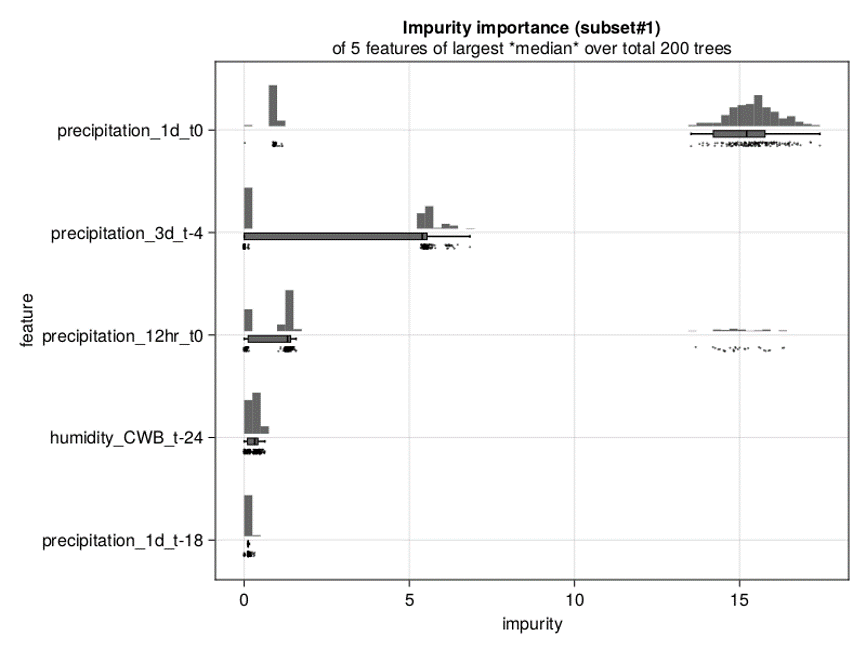
\includegraphics[width=0.5\textwidth]{Fig_impurityim.png}
    \end{center}
    \caption{ Impurity importance summarized from a trained forest model. \label{fig_impurityim}}
    %    \vspace{-8mm}
\end{figure}

By applying the ensemble model with the tree model as its atom, that is, the random forest algorithm, we show the statistics of the most important features in branching.
The tree is the approximator for the physical model of the soil-water dynamics.
The features near the root are the most important in prediction since the tree branches according to their values first.
Decision Tree algorithm partitions data into smaller datasets minimizing the heterogeneity of data in each dataset; thus, features used in the first few partitions are the most dominant decisions in the overall prediction process.
The dominance above can be quantified by summing the impurity differences in the whole process of branching; the features with highest impurity importance are summarized in Fig. \ref{fig_impurityim}. % FIXME: The description of impurity importance may be incorrect; you must check again.

\newpage


\subsection{Feature Importance (during testing)}

In contrast to impurity importance, Shapley value quantifies how a feature contributes to the prediction difference (comparing with the mean prediction); thus, features with higher Shapley values contribute to the prediction other than mean.




\newpage











\subsection{Analyzing the model}
The advantage of the tree algorithm is that we can inspect the trained model by plotting and analyzing the tree structure.

\newpage






\subsection{Performances over feature sets and depths}


In this section we investigate how a feature contributes to the performance further by applying training and k-folds cross validation over 12 feature sets.


\newpage




\section{Conclusion}
This is conclusion.
\newpage





%% The Appendices part is started with the command \appendix;
%% appendix sections are then done as normal sections
\appendix



%% If you have bibdatabase file and want bibtex to generate the
%% bibitems, please use
%%
\bibliographystyle{elsarticle-harv} % referst to elsarticle-harv.bst
\bibliography{main} % refers to main.bib
% KEYNOTE:
% For downloading the bst files: https://www.ctan.org/tex-archive/macros/latex/contrib/elsarticle

%% else use the following coding to input the bibitems directly in the
%% TeX file.






\end{document}

\endinput
%%
%% End of file `elsarticle-template-harv.tex'.
